%\VignetteEngine{knitr::knitr}
% some terminal commands to copy once and scroll when needed
% cd '/mnt/Hitachi2GB/00NMML/activePapers/KrigLinCaution/KrigLinCaution_package/KrigLinCaution/inst/doc'
% cd '/home/jay/Data/KrigLinCaution/KrigLinCaution_package/KrigLinCaution/inst/doc'
% Rscript -e "library(knitr); knit('KrigLinCaution.Rnw')"
% Rscript -e "library(knitr); purl('KrigLinCaution.Rnw')"
% pdflatex KrigLinCaution
% bibtex KrigLinCaution

\documentclass[11pt, titlepage]{article}\usepackage[]{graphicx}\usepackage[]{color}
%% maxwidth is the original width if it is less than linewidth
%% otherwise use linewidth (to make sure the graphics do not exceed the margin)
\makeatletter
\def\maxwidth{ %
  \ifdim\Gin@nat@width>\linewidth
    \linewidth
  \else
    \Gin@nat@width
  \fi
}
\makeatother

\definecolor{fgcolor}{rgb}{0.345, 0.345, 0.345}
\newcommand{\hlnum}[1]{\textcolor[rgb]{0.686,0.059,0.569}{#1}}%
\newcommand{\hlstr}[1]{\textcolor[rgb]{0.192,0.494,0.8}{#1}}%
\newcommand{\hlcom}[1]{\textcolor[rgb]{0.678,0.584,0.686}{\textit{#1}}}%
\newcommand{\hlopt}[1]{\textcolor[rgb]{0,0,0}{#1}}%
\newcommand{\hlstd}[1]{\textcolor[rgb]{0.345,0.345,0.345}{#1}}%
\newcommand{\hlkwa}[1]{\textcolor[rgb]{0.161,0.373,0.58}{\textbf{#1}}}%
\newcommand{\hlkwb}[1]{\textcolor[rgb]{0.69,0.353,0.396}{#1}}%
\newcommand{\hlkwc}[1]{\textcolor[rgb]{0.333,0.667,0.333}{#1}}%
\newcommand{\hlkwd}[1]{\textcolor[rgb]{0.737,0.353,0.396}{\textbf{#1}}}%
\let\hlipl\hlkwb

\usepackage{framed}
\makeatletter
\newenvironment{kframe}{%
 \def\at@end@of@kframe{}%
 \ifinner\ifhmode%
  \def\at@end@of@kframe{\end{minipage}}%
  \begin{minipage}{\columnwidth}%
 \fi\fi%
 \def\FrameCommand##1{\hskip\@totalleftmargin \hskip-\fboxsep
 \colorbox{shadecolor}{##1}\hskip-\fboxsep
     % There is no \\@totalrightmargin, so:
     \hskip-\linewidth \hskip-\@totalleftmargin \hskip\columnwidth}%
 \MakeFramed {\advance\hsize-\width
   \@totalleftmargin\z@ \linewidth\hsize
   \@setminipage}}%
 {\par\unskip\endMakeFramed%
 \at@end@of@kframe}
\makeatother

\definecolor{shadecolor}{rgb}{.97, .97, .97}
\definecolor{messagecolor}{rgb}{0, 0, 0}
\definecolor{warningcolor}{rgb}{1, 0, 1}
\definecolor{errorcolor}{rgb}{1, 0, 0}
\newenvironment{knitrout}{}{} % an empty environment to be redefined in TeX

\usepackage{alltt}
\usepackage{geometry}
\geometry{verbose,letterpaper,tmargin=2.54cm,bmargin=2.54cm,lmargin=2.54cm,rmargin=2.54cm}
\usepackage{graphicx, ams, amsmath, amssymb, natbib, setspace}
\usepackage{float}
\usepackage{multirow}
\usepackage{mathrsfs}
\usepackage{relsize}
\usepackage{subfigure}
\usepackage{pgf}
\usepackage{/mnt/Hitachi2GB/shTex/mymacros}
%\usepackage{/home/jay/Data/shTex/mymacros}
\usepackage{bbding}
\usepackage{lineno}
\usepackage{fancyvrb}
\usepackage[shortlabels]{enumitem}
\linenumbers
\setlength{\parindent}{3em}
%\onehalfspacing
\doublespacing
\usepackage{lipsum}
\usepackage{setspace}
\usepackage{etoolbox}
\AtBeginEnvironment{tabular}{\singlespacing}
\pdfpagewidth 8.5in
\pdfpageheight 11in
\setlength{\oddsidemargin}{0.0in} \setlength{\textwidth}{6.5in}
\setlength{\topmargin}{0.15in} \setlength{\textheight}{8.5in}
\setlength{\headheight}{0.0in} \setlength{\headsep}{0.0in}
%\renewcommand{\abstractname}{Summary}
%\renewcommand{\theequation}{(\arabic{equation})}
\setcounter{figure}{0}
\makeatletter
\renewcommand{\theequation}{eqn \arabic{equation}}
\renewcommand\tagform@[1]{\maketag@@@{\ignorespaces#1\unskip\@@italiccorr}}
\makeatother
\IfFileExists{upquote.sty}{\usepackage{upquote}}{}
\begin{document}


% ------------------------------------------------------------------------------
% ------------------------------------------------------------------------------
% 																	TITLE
% ------------------------------------------------------------------------------
% ------------------------------------------------------------------------------

\titlepage
\title {Kriging Models for Linear Networks and non-Euclidean Distances: Cautions, Solutions, and a Reanalysis of Ladle et al. (2016)}
\author{Jay M. Ver Hoef \\
\hrulefill \\ 
Marine Mammal Laboratory, NOAA-NMFS Alaska Fisheries Science Center\\
7600 Sand Point Way NE, Seattle, WA 98115\\
tel: (206) 201-2048 \hspace{.5cm} E-mail: jay.verhoef@noaa.gov\\
\hrulefill \\
}

\maketitle

% ------------------------------------------------------------------------------
% ------------------------------------------------------------------------------
% ------------------------------------------------------------------------------
% 														   	ABSTRACT
% ------------------------------------------------------------------------------
% ------------------------------------------------------------------------------
% ------------------------------------------------------------------------------
\renewcommand{\abstractname}{Summary}
\begin{abstract}
\begin{onehalfspace}

\begin{enumerate}
  \item There are now many examples where ecological researchers used non-Euclidean distance metrics in geostatistical models that were designed for Euclidean distance, such as those used for kriging.  This can lead to problems where predictions have negative variance estimates.  Technically, this occurs because the spatial covariance matrix, which depends on the geostatistical models, is not guaranteed to be positive definite when non-Euclidean distance metrics are used.
  \item I give a quick review of kriging and illustrate the problem with several fabricated examples, including locations on a circle, locations on a linear dichotomous network like streams, and locations on a linear trail or road network. I re-examine the linear network distance models from Ladle et al. (2016) and show that they are not guaranteed to have a positive definite covariance matrix.
  \item  I introduce the reduced rank method, also called a predictive process model, fixed-rank kriging, and a spatial basis function approach, for creating valid spatial covariance matrices with non-Euclidean distance metrics.  It has an additional advantage of fast computation for large data sets.
  \item I reanalyze the data of Ladle et al. (2016), showing that their fitted models, which used linear network distance in a geostatistical model without any nugget effect, had poor predictive performance compared to a model using Euclidean distance with a nugget effect, and it also had improper coverage for the prediction intervals. The reduced rank approach using linear network distances had the best predictive performance and had proper coverage for the prediction intervals.
\end{enumerate}
\end{onehalfspace}
\hrulefill \\

\noindent {\sc Key Words:} spatial statistics, geostatistics, prediction, reduced-rank methods, predictive process models\\

\end{abstract}

% ------------------------------------------------------------------------------
% ------------------------------------------------------------------------------
% ------------------------------------------------------------------------------
% 															INTRODUCTION
% ------------------------------------------------------------------------------
% ------------------------------------------------------------------------------
% ------------------------------------------------------------------------------

\newpage
\begin{spacing}{1.9}
\begin{flushleft}
\setlength{\parindent}{1cm}



\section*{INTRODUCTION}

There are now several examples in the ecological literature where, for spatial prediction like kriging, non-Euclidean distances were used in autocorrelation models developed under a Euclidean distance assumption.  This leads to a problem where prediction variances may be negative, and generally leads to unreliable prediction variances.  My objective is to help ecologists understand the problem and avoid this mistake.  In particular, I show the problems with extending kriging to linear networks advocated by \citet{Ladl:Avga:Whea:Boyc:pred:2016}, and reanalyze their data to show a better method for kriging on linear networks.

\subsection*{A Quick Review of Kriging}

Kriging is a method for spatial interpolation, beginning as a discipline of atmospheric sciences in Russia, of geostatistics in France, and appearing in English in the early 1960's \citep{Gand:obje:1963, Math:Prin:1963,Cres:orig:1990}.  Kriging is attractive because it has both predictions and prediction standard errors, providing uncertainty estimates for the predictions. Predictions and their standard errors are obtained after first estimating parameters of the kriging model.  The kriging model, like the familiar regression model, can be divided into two parts: 1) the non-stochastic part (also called the fixed effects, which includes covariates and regression parameters) and 2) the stochastic part (the random errors).  The ordinary kriging model is,
\begin{equation} \label{eq:OKmodel}
    Y_i = \mu + \varepsilon_i,
\end{equation}
where $Y_i$ is a spatial random variable at location $i$, $i = 1,2,\ldots,n$, with constant mean $\mu$ (the fixed effect) and random error $ \varepsilon_i$. In classical statistics, such as regression, the random errors are assumed to be independent from each other, with a single variance parameter.  For kriging, the independence assumption is relaxed, and the spatial distance among locations is used to model autocorrelation among random errors. Spatial autocorrelation is the tendency for spatial variables to co-vary, either in a similar fashion, or opposite from each other.  The most commonly observed spatial autocorrelation is when sites closer together tend to be more similar than those that are farther apart.  These tendencies are captured in autocorrelation and covariance matrices. 

Let $\bR$ be an autocorrelation matrix among spatial locations.  All of the diagonal elements of $\bR$ are ones. The $i$th row and $j$th column of the off-diagonal elements of $\bR$ are correlations, from minus one to one, between site $i$ and $j$.  Then a covariance matrix $\bC = \sigma^2_\textrm{p}\bR$ is just a scaled autocorrelation matrix that includes an overall variance, $\sigma^2_\textrm{p}$.  In constructing kriging models, practitioners often include a ``nugget'' effect, which is an independent (uncorrelated) random effect.  Constructing a full covariance matrix for a kriging model generally yields
\begin{equation} \label{eq:bSigma}
	\bSigma = \bC + \sigma^2_0\bI = \sigma^2_\textrm{p}\bR + \sigma^2_0\bI,
\end{equation}
where $\sigma^2_\textrm{p} \ge 0$ is called the partial sill, $\sigma^2_0 \ge 0$ is the nugget effect, and $\bI$ is the identity matrix (a diagonal matrix of all ones). The total variance is $\sigma^2_\textrm{p} + \sigma^2_0$.  The off-diagonal elements of $\bR$ are obtained from models that generally decrease as distance increases. Several autocorrelation models \citep[][p. 80--93]{Chil:Delf:geos:1999}, based on Euclidean distance, $d_{i,j}$, between sites $i$ and $j$, are
\begin{equation} \label{eq:autocorrModels}
	\begin{array}{l}
  \rho_{\textrm{e}}(d_{i,j}) = \exp(-d_{i,j}/\alpha), \\
  \rho_{\textrm{s}}(d_{i,j}) = [1 - 1.5(d_{i,j}/\alpha) + 0.5(d_{i,j}/\alpha)^3] \cI(d_{i,j} < \alpha), \\
  \rho_{\textrm{g}}(d_{i,j}) = \exp(-(d_{i,j}/\alpha)^2), \\
	\rho_{\textrm{c}}(d_{i,j}) = 1/(1+(d_{i,j}/\alpha)^2), \\
	\rho_{\textrm{h}}(d_{i,j}) = (\alpha/d_{i,j})\sin(d_{i,j}/\alpha)\cI(d_{i,j} > 0) + \cI(d_{i,j} = 0),
	\end{array}
\end{equation}
where distances are scaled by $\alpha \ge 0$, called the range parameter. $\cI(a)$ is an indicator function, equal to one if the argument $a$ is true, otherwise it is zero.

Examples of the autocorrelation models in \ref{eq:autocorrModels}, scaled with a partial sill, $\sigma^2_{\textrm{p}} = 2$, and a nugget effect, $\sigma^2_0 = 1$, are shown in Figure~\ref{fig:autocorrModels}a.  The exponential model, $\rho_{\textrm{e}}(d_{i,j})$, is a very popular model, and a special case of the Matern model.  It approaches zero autocorrelation asymptotically. The spherical model, $\rho_{\textrm{s}}(d_{i,j})$, is also very popular, and attains exactly zero autocorrelation at $\alpha$.  Both the exponential and spherical models decrease rapidly near the origin, for short distances, whereas the Gaussian model, $\rho_{\textrm{g}}(d_{i,j})$, decreases more slowly near the origin. This is also a special case of the Matern model, and creates very smooth spatial surfaces. The Cauchy model, $\rho_{\textrm{c}}(d_{i,j})$ is similar to the Gaussian, but approaches zero autocorrelation very slowly. Finally, The hole effect model, $\rho_{\textrm{h}}(d_{i,j})$ allows for negative autocorrelation in a dampened oscillating manner. These models highlight different features of autocorrelation models, and they will be used throughout this paper. Many more models are given in \citet[][p. 80--93]{Chil:Delf:geos:1999}.  

Kriging is often expressed as variograms and semivariograms.  Semivariograms model the variance of the \emph{difference} among variables. If $Y_i$ and $Y_j$ are random variables at spatial locations $i$ and $j$, respectively, a semivariogram is defined as $\gamma(d_{i,j}) \equiv \textrm{E}(Y_i - Y_j)^2/2$, where E is expectation.  All of the models in \ref{eq:autocorrModels} can be written as semivariograms,
\begin{equation} \label{eq:semivarrho}
				\gamma_m(d_{i,j}) = \sigma^2_\textrm{p}(1 - \rho_m(d_{i,j})),
\end{equation}
where $m$ = e, s, g, c, or h for exponential, spherical, Gaussian, Cauchy, or hole effect, respectively. Figure~\ref{fig:autocorrModels}b shows semivariograms that are equivalent to the models in Figure~\ref{fig:autocorrModels}a.  A matrix of semivariogram values among spatial locations can be written in terms of \ref{eq:bSigma},
\[
\bGamma = (\sigma_0^2 + \sigma^2_{\textrm{p}})\bI - \bSigma.
\]

Autocorrelation needs to be estimated from data. Empirical semivariograms have been used since the origins of kriging. First, all pairwise distances are binned into distance classes, $\cD_k = [h_{k-1},h_k)$, where $0 \le h_0 < h_1$ and $h_{k-1} < h_k$ for $k = 1, 2, \ldots, K$, that partition the real line into mutually exclusive and exhaustive segments that cover all distances in the data set.  Then the empirical semivariogram is,
\[
				\hat{\gamma}(h_k) = \frac{1}{2N(\cD_k)}\sum_{d_{i,j} \in \cD_k} (y_i - y_j)^2,
\]
for all possible pairs of $i$ and $j$, and $k = 1, \ldots, K$, where $y_1, . . . ,y_n$ are the observed data, $h_k$ is a representative distance (often the average or midrange) for a distance bin $\cD_k$, and $N(\cD_k)$ is the number of distinct pairs in $\cD_k$. Empirical semivariograms have desirable estimation properties \citep[it is an unbiased estimator,][p. 71]{Cres:stat:1993} because, substituting \ref{eq:OKmodel} into the semivariogram definition, $\mu$ cancels, obviating the need to estimate it.  To estimate autocorrelation, one of the models in \ref{eq:autocorrModels}, in semivariogram form, \ref{eq:semivarrho}, can be fit to $\hat{\gamma}(h_k)$ as a function of $h_k$, often using weighted least squares \citep{Cres:fitt:1985}.  This concept is generalized by restricted maximum likelihood \citep[REML, ][]{Patt:Thom:reco:1971, Patt:Thom:maxi:1974}, which can be used for autocorrelation in regression models with several covariates and regression coefficients \citep[for REML applied to spatial models, see, e.g.,][p. 93]{Cres:stat:1993}. In addition, REML eliminates the arbitrary binning of distances for variogram estimation.  Although REML was originally derived assuming normality, REML can be viewed as unbiased estimating equations \citep{Heyd:quas:1994, Cres:Lahi:asym:1996}, so normality is not required to estimate covariance parameters.  Later, I will use REML for estimation. Also, I focus on covariances, rather than variograms, because their interpretation is more readily understood in the broader context of statistical models.

After covariance parameters are estimated from the data, kriging is the spatial prediction (interpolation) for spatial locations where data were not collected.  Kriging provides best linear unbiased predictions (BLUP) in the sense of minimizing the expected squared errors between the data as predictors, and the predictand, subject to unbiasedness (on average). The ordinary kriging prediction equations, in terms of the covariance matrix \citep[][p.33]{Scha:Gotw:stat:2005}, are
\begin{equation} \label{eq:OK}
	\hat{Y}_{n+\ell} = \hat{\mu} + \bc\upp\bSigma\upi(\by - \bone\hat{\mu}), 
\end{equation}
for $M$ predictions with locations indexed by $n+\ell$, $\ell = 1,2,\ldots,M$. Here, $\bone$ is a vector of ones, $\hat{\mu} = (\bone\upp\bSigma\upi\by)/(\bone\upp\bSigma\upi\bone)$, and $\bc$ has, as its $i$th element, $\sigma^2_p\rho_m(d_{i,n+\ell})$, where $m$ is the same model (one of those in \ref{eq:autocorrModels}) that was used in $\bSigma$. The prediction variance (the expected squared errors that were minimized) is given by
\begin{equation} \label{eq:OKse}
	\var(\hat{Y}_{n+\ell}) = (\sigma^2_p + \sigma^2_0) - \bc\upp\bSigma\upi\bc + \frac{(1 - \bone\upp\bSigma\upi\bc)^2}{\bone\upp\bSigma\upi\bone}
\end{equation}


\subsection*{The Problem}

One of the properties shared by all models in \ref{eq:autocorrModels} is that, when $d_{i,j}$ is Euclidean distance, the covariance matrix in \ref{eq:bSigma} is guaranteed to be positive definite for all possible spatial configurations of points (in 3 dimensions or less) and all possible parameter values:  $\sigma^2_\textrm{p} \ge 0, \sigma^2_0 \ge 0$, and $\alpha \ge 0$ (one of $\sigma^2_\textrm{p}$ or $\sigma^2_0$ must be greater than zero). It is important for $\bSigma$ to be positive definite because many estimators and predictors in statistics are linear functions of the data, kriging being one of them.  That is, let $\bomega$ be a vector of weights and $\by$ be a vector of random variables with covariance matrix $\bSigma$.  Then an estimator or predictor $\hat{T} = \bomega\upp\by$ will have variance
\begin{equation} \label{eq:quadForm}
  \var(\hat{T}) = \bomega\upp\bSigma\bomega,
\end{equation}
which is guaranteed to be positive only if $\bSigma$ is positive definite \citep{Guil:Schi:Porc:Bevi:vali:2014}.  Requiring $\bSigma$ to be positive definite is the matrix analog of requiring a variance parameter to be positive. For example, \citet{Guil:Schi:Porc:Bevi:vali:2014} demonstrate that the triangle model (not given in \ref{eq:autocorrModels}), which is only valid in one dimension, yields negative variances when used with Euclidean distances based on locations in two-dimensions.

The simplest way to check whether a matrix is positive definite is to check the eigenvalues of that matrix.  A covariance matrix $\bSigma$ should be composed of real values, and it should be symmetric.  Then 
\begin{equation} \label{eq:spectralDecomp}
  \bSigma = \bQ\bLambda\bQ\upp
\end{equation}
is called the spectral decomposition of $\bSigma$, where each column of $\bQ$ contains an eigenvector, and the corresponding eigenvalue is contained in $\bLambda$, which is a diagonal matrix.  Substituting \ref{eq:spectralDecomp} into \ref{eq:quadForm} gives
\[
\var(\hat{T}) = \bv\upp\bLambda\bv = \sum_{i=1}^n v_i^2\lambda_i
\]
where $\bv = \bQ\upp\bomega$. Because $v_i^2 \ge 0$, $\var(\hat{T})$ is guaranteed to be positive as long as all $\lambda_i$ are greater than zero and at least one $v_i^2$ is greater than zero.  So, if the smallest eigenvalue of $\bSigma$ is greater than zero, then $\bSigma$ is positive definite.

Now consider using the models in \ref{eq:autocorrModels} for cases where $d_{i,j}$ is non-Euclidean.  For example, let 11 spatial locations occur at equal distances on a circle (Figure~\ref{fig:cautionEx}a).  Let distance be defined as the shortest path distance, so that two adjacent points have distance $2\pi/11$, and the maximum distance between any two points is $10\pi/11$.  The $11 \times 11$ distance matrix was used with autocorrelation models in \ref{eq:autocorrModels}, and the minimum eigenvalue is plotted in Figure~\ref{fig:cautionEx}b.  Notice that as the range parameter $\alpha$ increases, the hole effect, Gaussian, and Cauchy models have a minimum eigenvalue that is less than zero, so for these values of $\alpha$, the matrix is not positive definite, and cannot be a covariance matrix. This example points out a further problem.  It appears that the exponential model and spherical model are valid models for all range values; however, this is only true for 11 points that are equidistant apart.  There is no guarantee that the exponential and spherical model will provide positive definite covariance matrices for other sample sizes and other spatial configurations.  Later, I will discuss more general approaches for developing models for all spatial configurations and all values of the range parameter.

Another example is provided by the spatial locations at the nodes of a dichotomous network (Figure~\ref{fig:cautionEx}c). The distance between each location and the nearest node is exactly one, and there are $2^7 - 1$ locations.  Again, let distance be defined as the shortest path between any two locations, so the maximum distance between two terminal locations is $2 \times 6 = 12$.  Using the $127 \times 127$ distance matrix with the autocorrelation models in \ref{eq:autocorrModels} for various $\alpha$ values showed that all models yielded minimum eigenvalues below zero except the exponential model (Figure~\ref{fig:cautionEx}d).  The hole effect model illustrates how erratic the positive definite condition can be, where small changes in $\alpha$ cause wild swings on whether the covariance matrix is positive definite. An argument on why the exponential model is always positive definite for the dichotomous network situation is given by \citet{Ver:Pete:Move:2010}.

Finally, consider the 25 locations in Figure~\ref{fig:cautionEx}e.  This is representative of a road or trail system on a perfectly regular grid.  Again, consider the shortest path distance between any two points.  First, consider the situation where sites are only connected by the solid lines.  In that case, sites one and two are not connected directly, but rather the distance between them is 3 (through sites 6 and 7).  Using the $25 \times 25$ distance matrix with the autocorrelation models in \ref{eq:autocorrModels} for various $\alpha$ values shows that none of the models are positive definite for all $\alpha$ (Figure~\ref{fig:cautionEx}f). A variation occurs if we let the sites with dotted lines be connected, as well as those with solid lines.  In this case, the exponential model remains positive definite for all values of $\alpha$, and an explanation is provided by \citet{Curr:NonE:2006}.

Figure~\ref{fig:cautionEx} demonstrates that, in a variety of situations, models that guarantee positive definite covariance matrices for any spatial configuration, and any range value $\alpha > 0$, when using Euclidean distance, no longer guarantee positive definite matrices when using linear network distances. Similarly, one might wonder why we do not use empirical covariances in $\bSigma$.  That is, let the $i,j$ entry in $\bSigma$ be $(y_i - \hat{\mu})(y_j - \hat{\mu})$, where $\hat{\mu}$ is the average of all $y_i$.  Again, there is no guarantee that $\bSigma$ will be positive definite.  If it is not, then what is the analyst to do? Geostatistics has a long tradition of only considering models that guarantee positive definite matrices \citep[][p. 161]{Jour:Huij:mini:1978}. For example, \citet[][p. 80]{Webs:Oliv:geos:2007} call them ``authorized'' models, while \citet[][p. 87]{Goov:geos:1997} calls them ``permissible'' models.  All of the models in \ref{eq:autocorrModels} are permissible for Euclidean distance in three dimensions or less, but they are clearly not generally permissible for linear network distances.

\subsection*{Literature Review}

Many authors have used autocovariance models, such as those in \ref{eq:autocorrModels}, with non-Euclidean distances, and they have been roundly criticized \citep{Curr:NonE:2006}.  For example, for streams, impermissible models have been used by \citet{Cres:Maju:spat:1997} and \citet{Gard:Sull:Lemb:pred:2003}, who substituted in-stream distance for Euclidean distance, and in fact this same idea was recommended in \citet{Okab:Sugi:spat:2012}. Alternatively, permissible models that guarantee positive-definite covariance matrices were developed (based on a spatial moving averages, a spatially continuous analog of moving average models in times series) by \citet{Ver:Pete:Theo:spat:2006}, \citet{Cres:Frey:Harc:Smit:spat:2006} and \citet{Ver:Pete:Move:2010}. 

For roads and trails, impermissible models have been used by \citet{Shio:Shio:stre:2011}, \citet{Selb:Kock:spat:2013} and \citet{Ladl:Avga:Whea:Boyc:pred:2016}, who substitute network-based distance for Euclidean distance.  However, the exponential is a permissible model for a perfect grid using Manhattan distance (as described for Figure~\ref{fig:cautionEx}e); see \citet{Curr:NonE:2006}. I provide a more general approach based on reduced-rank radial-basis functions below. 

In estuaries, shortest-path distances were used to replace Euclidean distance in \citet{Litt:Edwa:Port:krig:1997}, \citet{Rath:spat:1998}, and \citet{Jens:Chri:Mill:land:2006}, which yields impermissible models.  Instead, permissible models based on reduced-rank radial-basis functions were given by \citet{Wang:Rana:low:2007}.  

There has been a great deal of interest in kriging over the surface of the earth, which is an approximate sphere.  Kriging on geographical coordinates can create distortions, yet such applications have appeared \citep{Ecke:Gelf:baye:1997,Kalu:Vega:Card:Shel:anal:1998}, which have been criticized \citep{Bane:geod:2005}. Most research has centered on geodesic, or great-circle distance. If geodesic distance is substituted for Euclidean distance for the models in \ref{eq:autocorrModels}, only the exponential and spherical models are permissible \citep{Gnei:stri:2013}.  Note that distance is measured in radians, and restricted to the interval $[0,\pi]$.

For an interesting ecological application, \citet{Brad:Ralp:Coop:dise:2013} propose an extension of a powered exponential, also called a stable geostatistical model, that combines Euclidean distance with ecological or genetic distance. Then \citet{Guil:Schi:Porc:Bevi:vali:2014} show how the stable model can be used with geodesic (great circle) distances, but only if the power parameter of the stable model is restricted, and they also discuss ways of ``gluing'' geographical distances and environmental distances to create permissible models.

The literature given above, with many examples, shows that replacing Euclidean distance with some other metric that makes more physical sense is intuitively appealing, but may lead to covariance functions that do not guarantee positive definite covariance matrices. I will discuss this further after a re-analysis of the data in \citet{Ladl:Avga:Whea:Boyc:pred:2016}. 

%%%%%%%%%%%%%%%%%%%%%%%%%%%%%%%%%%%%%%%%%%%%%%%%%%%%%%%%%%%%%%%%%%%%%%%%%%%%%%%%
%%%%%%%%%%%%%%%%%%%%%%%%%%%%%%%%%%%%%%%%%%%%%%%%%%%%%%%%%%%%%%%%%%%%%%%%%%%%%%%%
%                         loadLibrary Chunk
%%%%%%%%%%%%%%%%%%%%%%%%%%%%%%%%%%%%%%%%%%%%%%%%%%%%%%%%%%%%%%%%%%%%%%%%%%%%%%%%
%%%%%%%%%%%%%%%%%%%%%%%%%%%%%%%%%%%%%%%%%%%%%%%%%%%%%%%%%%%%%%%%%%%%%%%%%%%%%%%%



%%%%%%%%%%%%%%%%%%%%%%%%%%%%%%%%%%%%%%%%%%%%%%%%%%%%%%%%%%%%%%%%%%%%%%%%%%%%%%%%
%%%%%%%%%%%%%%%%%%%%%%%%%%%%%%%%%%%%%%%%%%%%%%%%%%%%%%%%%%%%%%%%%%%%%%%%%%%%%%%%
%                         autocorrModels Chunk
%%%%%%%%%%%%%%%%%%%%%%%%%%%%%%%%%%%%%%%%%%%%%%%%%%%%%%%%%%%%%%%%%%%%%%%%%%%%%%%%
%%%%%%%%%%%%%%%%%%%%%%%%%%%%%%%%%%%%%%%%%%%%%%%%%%%%%%%%%%%%%%%%%%%%%%%%%%%%%%%%



%%%%%%%%%%%%%%%%%%%%%%%%%%%%%%%%%%%%%%%%%%%%%%%%%%%%%%%%%%%%%%%%%%%%%%%%%%%%%%%%
%%%%%%%%%%%%%%%%%%%%%%%%%%%%%%%%%%%%%%%%%%%%%%%%%%%%%%%%%%%%%%%%%%%%%%%%%%%%%%%%
%                         CautionEx Chunk
%%%%%%%%%%%%%%%%%%%%%%%%%%%%%%%%%%%%%%%%%%%%%%%%%%%%%%%%%%%%%%%%%%%%%%%%%%%%%%%%
%%%%%%%%%%%%%%%%%%%%%%%%%%%%%%%%%%%%%%%%%%%%%%%%%%%%%%%%%%%%%%%%%%%%%%%%%%%%%%%%



%%%%%%%%%%%%%%%%%%%%%%%%%%%%%%%%%%%%%%%%%%%%%%%%%%%%%%%%%%%%%%%%%%%%%%%%%%%%%%%%
%%%%%%%%%%%%%%%%%%%%%%%%%%%%%%%%%%%%%%%%%%%%%%%%%%%%%%%%%%%%%%%%%%%%%%%%%%%%%%%%
%                         realLinDistEigVals Chunk
%%%%%%%%%%%%%%%%%%%%%%%%%%%%%%%%%%%%%%%%%%%%%%%%%%%%%%%%%%%%%%%%%%%%%%%%%%%%%%%%
%%%%%%%%%%%%%%%%%%%%%%%%%%%%%%%%%%%%%%%%%%%%%%%%%%%%%%%%%%%%%%%%%%%%%%%%%%%%%%%%




%%%%%%%%%%%%%%%%%%%%%%%%%%%%%%%%%%%%%%%%%%%%%%%%%%%%%%%%%%%%%%%%%%%%%%%%%%%%%%%%
%%%%%%%%%%%%%%%%%%%%%%%%%%%%%%%%%%%%%%%%%%%%%%%%%%%%%%%%%%%%%%%%%%%%%%%%%%%%%%%%
%                         reduRank Chunk
%%%%%%%%%%%%%%%%%%%%%%%%%%%%%%%%%%%%%%%%%%%%%%%%%%%%%%%%%%%%%%%%%%%%%%%%%%%%%%%%
%%%%%%%%%%%%%%%%%%%%%%%%%%%%%%%%%%%%%%%%%%%%%%%%%%%%%%%%%%%%%%%%%%%%%%%%%%%%%%%%



%%%%%%%%%%%%%%%%%%%%%%%%%%%%%%%%%%%%%%%%%%%%%%%%%%%%%%%%%%%%%%%%%%%%%%%%%%%%%%%%
%%%%%%%%%%%%%%%%%%%%%%%%%%%%%%%%%%%%%%%%%%%%%%%%%%%%%%%%%%%%%%%%%%%%%%%%%%%%%%%%
%                         rrFits Chunk
%%%%%%%%%%%%%%%%%%%%%%%%%%%%%%%%%%%%%%%%%%%%%%%%%%%%%%%%%%%%%%%%%%%%%%%%%%%%%%%%
%%%%%%%%%%%%%%%%%%%%%%%%%%%%%%%%%%%%%%%%%%%%%%%%%%%%%%%%%%%%%%%%%%%%%%%%%%%%%%%%



%%%%%%%%%%%%%%%%%%%%%%%%%%%%%%%%%%%%%%%%%%%%%%%%%%%%%%%%%%%%%%%%%%%%%%%%%%%%%%%%
%%%%%%%%%%%%%%%%%%%%%%%%%%%%%%%%%%%%%%%%%%%%%%%%%%%%%%%%%%%%%%%%%%%%%%%%%%%%%%%%
%                         CVplots Chunk
%%%%%%%%%%%%%%%%%%%%%%%%%%%%%%%%%%%%%%%%%%%%%%%%%%%%%%%%%%%%%%%%%%%%%%%%%%%%%%%%
%%%%%%%%%%%%%%%%%%%%%%%%%%%%%%%%%%%%%%%%%%%%%%%%%%%%%%%%%%%%%%%%%%%%%%%%%%%%%%%%



% ------------------------------------------------------------------------------
% ------------------------------------------------------------------------------
% ------------------------------------------------------------------------------
% 								REANALYSIS OF LADLE ET AL. (2016)
% ------------------------------------------------------------------------------
% ------------------------------------------------------------------------------
% ------------------------------------------------------------------------------

\section*{REANALYSIS OF LADLE ET AL. (2016)}

Prior to a reanalysis of \citet{Ladl:Avga:Whea:Boyc:pred:2016}, I review their analysis.  I then review several general approaches to spatial models for non-Euclidean distance metrics. Finally, I introduce the reduced rank method that I ultimately use on the data of \citet{Ladl:Avga:Whea:Boyc:pred:2016}.

\subsection*{Review of Ladle et al. (2016)}

\citet{Ladl:Avga:Whea:Boyc:pred:2016} fit models without a nugget effect, justifying the decision based on a prior belief that no nugget was present. Examination of Fig. 2 in \citet{Ladl:Avga:Whea:Boyc:pred:2016} would lead most spatial statistical modelers to include a nugget effect because a visual extrapolation to the origin leads to a discontinuity from zero.  Moreover, when variograms are fitted without a nugget effect, they should be checked carefully for fitting and prediction instabilities. It is well-known that models without nugget can lead to computational instability when inverting the covariance matrix \citep{Diam:Arms:robu:1984,Posa:cond:1989,ODow:cond:1991,Abab:cond:1994}. If the modeler insists on excluding the nugget effect \citep[as often occurs when using kriging to approximate deterministic computer models, e.g.][]{Mart:Simp:krig:2005}, a small nugget effect can be added to the diagonal (e.g. $1 \times 10^-6$ was used in \citet{Book:Denn:Fran:Sera:etal:rigo:1999}) to improve computational stability.  Problems can occur due to model type (Gaussian autocorrelation is the worst) and the arrangement of the spatial locations, when ``near duplicate'' locations can cause apparently singular matrices for computational purposes \citep[][p. 220]{Biva:Pebe:Gome:appl:2008}.

The main objective of this paper, and my prior review, is that substitution of non-Euclidean distance metrics into autocorrelation models derived for Euclidean distance can create covariance matrices that are not positive definite. For the particular case of \citet{Ladl:Avga:Whea:Boyc:pred:2016}, using their linear-network distance matrix in the models given in \ref{eq:autocorrModels} showed that none of the models are permissible beyond a certain $\alpha$ value (Figure~\ref{fig:realLinDistEigVals}a).  On the other hand, using the Euclidean distance matrix provided by Ladle et al. (2016), all models yield positive-definite covariance matrices at all values of $\alpha > 0$ (Figure~\ref{fig:realLinDistEigVals}b), which simply verifies that they are permissible models.  Note that the fitted exponential model had $\hat{\alpha} = 7620$ in \citet{Ladl:Avga:Whea:Boyc:pred:2016} for motorised and $\hat{\alpha} = 14245$ for nonmotorised variables, which yielded positive definite covariance matrices because $\alpha <$ 28224 had all positive eigenvalues (Figure~\ref{fig:realLinDistEigVals}a). The (incorrectly) fitted spherical models in \citet{Ladl:Avga:Whea:Boyc:pred:2016} had estimated range parameters $>40,000$, which would not yield positive-definite covariance matrices because $\alpha >$ 15876 had negative eigenvalues (Figure~\ref{fig:realLinDistEigVals}a).

\subsection*{Review of Non-Euclidean Distance Models}

I will review two general approaches for creating spatial models in novel situations, whether for non-Euclidean distances or other situations.  The first is the spatial moving average, also called a process convolution and autoconvolution.  The spatial moving average approach is very similar to a moving average model in time series, except that the random variables that are ``smoothed'' are continuous in space (also known as a white noise process).  This approach has been used for flexible variogram modeling \citep{Barr:Ver:blac:1996}, multivariable (cokriging) models \citep{Ver:Barr:cons:1998,Ver:Cres:Barr:flex:2004}, nonstationary models \citep{Higd:proc:1998,Higd:Swal:Kern:non-:1999}, stream network models \citep{Ver:Pete:Theo:spat:2006, Cres:Frey:Harc:Smit:spat:2006, Ver:Pete:Move:2010}, models on the sphere \citep{Gnei:stri:2013}, and spatio-temporal models \citep{Wikl:kern:2002,Conn:John:Ver:spat:2015}. Using the moving average approach requires solving integrals to obtain the autocorrelation function, or approximating the integrals. For example, the integrals are tractable for stream networks when purely dichotomous branching occurs \citep{Ver:Pete:Theo:spat:2006}, however they are not tractable for more general linear networks. 

The second approach is a reduced rank idea, also called a dimension reduction \citep{Wikl:Cres:dime:1999} and spatial radial basis \citep{Lin:Chen:spat:2004, Hefl:Brom:Bros:Bude:basi:2016} method, which handles non-Euclidean topology and has computational advantages.  This is a very general method, and the one that I will use to re-analyze the data of \citet{Ladl:Avga:Whea:Boyc:pred:2016}.  It has been used for shortest path distances in estuaries \citep{Wang:Rana:low:2007}, but it is mostly featured as a method for big data sets \citep[e.g.][]{Wikl:Cres:dime:1999, Rupp:Wand:Carr:semi:2003, Cres:Gard:fixe:2008,Bane:Gelf:Finl:Sang:gaus:2008}.  I will use this method for models using linear network distances, which I describe next.


\subsection*{Reduced Rank Methods for Non-Euclidean Distances}

The reduced rank models are a special case of linear mixed models, so I provide a quick review. In fact, \ref{eq:OKmodel} is a special case of a mixed model. A mixed model is often written as
\begin{equation} \label{eq:mixedMod}
    \by = \bX\bbeta + \bZ\bgamma + \bvarepsilon,
\end{equation}
 where $\bX$ is a design matrix with covariates, $\bbeta$ is a vector of regression parameters, $\bZ$ is a random-effects design matrix, $\bgamma$ is a vector of zero-mean random effects with variance $\sigma^2_\textrm{p}$, and $\var(\bvarepsilon) = \sigma^2_0 \bI$.  In statistical textbooks, $\bZ$ in \ref{eq:mixedMod} often contains dummy variables (zeros or ones) that indicate some factor level of the random effect.  However, $\bZ$ can also contain covariates, in which case $\bgamma$ contains random effects for the slope of a line, illustrating that there are no restrictions on the types of values (continuous or categorical) contained in $\bZ$. For the linear mixed model, \ref{eq:mixedMod}, recall that
 \begin{equation} \label{eq:varMixedMod}
 \var(\by) = \sigma^2_\textrm{p}\bZ\bG\bZ\upp + \sigma^2_0\bI, 
 \end{equation}
 where $\bG$ is the correlation matrix for $\bgamma$.  Classically, for mixed models, random effects are assumed independent, so $\bG = \bI$, and then $\var(\by) = \sigma^2_\textrm{p}\bZ\bZ\upp + \sigma^2_0\bI$.  

 For the reduced rank models, let $\bD$ denote a matrix of Euclidean distances among locations and $\bL$ denote a matrix of linear network distances. Let $\bR_{m,\bA,\alpha}$ be a spatial autocorrelation matrix, where $m$ = e, s, g, c, or h, for exponential, spherical, Gaussian, Cauchy, or hole effect, respectively, for one of the models in \ref{eq:autocorrModels}, $\bA$ is a distance matrix, either $\bD$ or $\bL$, and $\alpha$ is the range parameter for one of the models in \ref{eq:autocorrModels}.  For example, $\bR_{\textrm{e},\bL,\alpha} = \exp(-\bL/\alpha)$.  Then let $\bR^r_{m,\bA,\alpha}$ be the matrix where some of the columns of $\bR_{m,\bA,\alpha}$ are kept as ``knots'', and all other columns have been removed; hence the term ``reduced rank.''  For example, for the Ladle et al. (2016) data, there are 239 locations, so $\bR_{m,\bA,\alpha}$ is $239 \times 239$. I will reduce it to just 120 columns, so $\bR^r_{m,\bA,\alpha}$ is $239 \times 120$.  

The reduced rank method requires the selection of knots.  In general, knots can be placed anywhere, and not only at the observed locations.  I used K-means clustering \citep{MacQ:some:1967} on the spatial coordinates to create 120 groups. Because K-means clustering minimizes within-group variance while maximizing among-group variance, the centroid of each group tends to be regularly spaced; i.e. it is a space-filling design \citep[e.g.][]{Ver:Jans:esti:2015}.  Then, the knots were moved to the nearest observed location. The original knot locations are shown in blue, and then moved to the red circles in Fig.~\ref{fig:reduRank}.  It will be useful to have the matrix of Euclidean distances among knots only, which is a subset of the rows and columns of $\bD$, and I denote the knot-to-knot distances as $\bD^k$. 

Now consider the following random effects model as a special case of \ref{eq:mixedMod},
\begin{equation} \label{eq:RRmodel}
	\by = \bone\mu + [\bR^r_{m,\bA,\alpha}]\bgamma + \bvarepsilon,
\end{equation}
In \ref{eq:RRmodel}, I have replaced $\bZ$ with $\bR_{m,\bA,\alpha}^r$, and there are no covariates in $\bX$, so $\bX$ is a vector of ones, and I will assume that $\var(\bgamma)=[\bR_{m,\bD^k,\eta}]\upi$.  A broad introduction to spatial basis functions, and rank reduction, for ecologists is given by \citet{Hefl:Brom:Bros:Bude:basi:2016}.

The innovations for reduced-rank spatial models in \ref{eq:RRmodel} occur because: 1) we use correlation models of distance in the random effects design matrix, essentially $\bZ = \bR^r_{m,\bA,\alpha}$, and 2) we also allow the random effects $\bgamma$ to be spatially autocorrelated using the \emph{inverse} covariance matrix from one of the models in \ref{eq:autocorrModels}.  The model in \ref{eq:RRmodel} must have a positive definite covariance matrix, so I assume Euclidean distance will be used for the distance among knots.  In that case, \ref{eq:RRmodel} leads to the following covariance matrix,
\begin{equation} \label{eq:varRR}
				\bSigma = \sigma^2_\textrm{p}\bR^r_{m,\bA,\alpha}[\bR_{m,\bD^k,\eta}]\upi[\bR^r_{m,\bA,\alpha}]\upp + \sigma^2_0\bI
\end{equation}
In fact, each model subscript $m$ in \ref{eq:varRR} could be different, and $\bA$ could be either $\bD$ or $\bL$, or some other matrix based on any number of distance metrics.  The construction \ref{eq:varRR} is very flexible, and several comments are pertinent:
\begin{enumerate}
		\item Strictly speaking, the covariance matrix in \ref{eq:varRR} is guaranteed to be positive definite only if $\sigma_0^2 > 0$. This is no different than mixed models, \ref{eq:mixedMod}, where recall that the variance was $\sigma^2_\textrm{p}\bZ\bG\bZ\upp + \sigma_0^2\bI$.  
		\item Note that the inverse of a positive definite matrix will also be positive definite, so $[\bR_{m,\bD^k,\eta}]\upi$ is positive definite as long as Euclidean distance $\bD^k$ is used.  That ensures that $\sigma^2_\textrm{p}\bR^r_{m,\bA,\alpha}[\bR_{m,\bD^k,\eta}]\upi[\bR^r_{m,\bA,\alpha}]\upp$ is nonnegative definite.
		\item It might seem unusual to model the covariance among the knots as the inverse $[\bR_{m,\bD^k,\eta}]\upi$. The reasons for the inverse are complex \citep{Bane:Gelf:Finl:Sang:gaus:2008},  but there is an intuitive explanation.  Suppose that the reduced rank matrix is based on Euclidean distance, that is, let $\bA = \bD$, so we have $\bR^r_{m,\bD,\alpha}$. Now, let the knots increase in number until the knots become exactly the same as the observed locations. Then, $\bR^r_{m,\bD,\alpha}$ becomes $\bR_{m,\bD,\alpha}$, the full covariance matrix, and $[\bR_{m,\bD^k,\eta}]\upi$ becomes $[\bR_{m,\bD,\alpha}]\upi$, the inverse of the full covariance matrix. The inverse cancels one of the full covariance matrices, so in \ref{eq:varRR}, $\sigma^2_\textrm{p}\bR_{m,\bD,\alpha}[\bR_{m,\bD,\alpha}]\upi[\bR_{m,\bD,\alpha}]\upp = \sigma^2_\textrm{p}\bR_{m,\bD,\alpha}$, which is the $n \times n$ symmetric covariance matrix without any reduction in rank.  By using the inverse, the formulation in \ref{eq:varRR} allows us to recover a typical covariance matrix as the knots become equal to the observed locations.  My approach will be that $\bG$ in \ref{eq:mixedMod} is $[\bR_{m,\bD^k,\eta}]\upi$, but note that any other positive definite matrix could be used for $\bG$, including $\bG = \bI$.
		\item It is not necessary to use reduced rank.  The full covariance matrices in \ref{eq:varRR} could be used, including the inverse if the Euclidean-distance covariance matrix sandwiched between the linear-distance covariance matrices, but see the next item.
		\item In addition to allowing non-Euclidean distances in the random-effects design matrix, $\bR^r_{m,\bA,\alpha}$, there is a computational advantage to using rank reduction in \ref{eq:varRR}.  Notice that $\bSigma$ is a $239 \times 239$ matrix, and likelihood based methods (such as maximum likelihood, or restricted maximum likelihood) require the inverse of $\bSigma$.  Computing matrix inverses is computationally expensive, and grows exponentially with the dimension of the matrix (as a cube of the number of locations).  However, the reduced rank formulation allows an inverse of $\bSigma$ that is reduced to the size of the rank reduction by using the Sherman-Morrison-Woodbury result \citep{Sher:Morr:adju:1949,Wood:inve:1950}; see an excellent review by \citet{Hend:Sear:on:1981}. In our case, if we choose 120 knots, then the inverse would be for a $120 \times 120$ matrix rather than a $239 \times 239$ matrix.
		
\end{enumerate}

In what follows, I will always choose a single model form, $m$, across all 3 components of $\bR^r_{m,\bA,\alpha}[\bR_{m,\bD^k,\eta}]\upi[\bR^r_{m,\bA,\alpha}]\upp$, and I will always use the linear network distance matrix $\bL$ for $\bA$, but allow the autocorrelation parameter $\alpha$ to be different from $\eta$.  For example, the reduced rank exponential model that uses linear network distance has a covariance matrix
\begin{equation} \label{eq:RRmodCov}
				\bSigma = \sigma^2_\textrm{p}\bR^r_{\textrm{e},\bL,\alpha}[\bR_{\textrm{e},\bD^k,\eta}]\upi[\bR^r_{\textrm{e},\bL,\alpha}]\upp + \sigma^2_0\bI.
\end{equation}
For this covariance matrix, there are 4 parameters to estimate; $\sigma^2_\textrm{p}$, $\alpha$, $\eta$, and $\sigma^2_0$.  In what follows, I fit all reduced rank models using REML.

\subsection*{Reanalysis of the Ladle et al. (2014) Data}

The reanalysis of \citet{Ladl:Avga:Whea:Boyc:pred:2016} is given in Table~\ref{Tab:CVstats}. The data were downloaded from the Dryad Repository http://dx.doi.org/10.5061/dryad.62t17.  The parameter estimates for the two exponential models found in \citet{Ladl:Avga:Whea:Boyc:pred:2016} for motorised and nonmotorised variables are given in the first row.  To evaluate models, I use four criteria, the first being AIC \citep{Akai:Info:1973,Burn:Ande:mode:2002}, which assumes that the data were distributed as a multivariate normal likelihood with a spatial covariance matrix \citep[for an example using spatial models, see][]{Hoet:Davi:Mert:Thom:mode:2006}.   

The rest of the criteria are based on leave-one-out crossvalidation.  Let $\by_{-i}$ be the vector of observed data with the $i$th observation removed. Then, using $\by_{-i}$ and the estimated covariance matrix, with the $i$th row and column removed, the $i$th observation is predicted, denoted as $\hat{y}_i$,  with \ref{eq:OK}, and its prediction standard error, denoted as $se(\hat{y}_i$), is estimated with \ref{eq:OKse}. The correlation was computed on the set $\{y_i,\hat{y}_i\}$ for all $i$ and reported as Corr in Table~\ref{Tab:CVstats}.  Root-mean-squared prediction error (RMSPE, Table~\ref{Tab:CVstats}) was computed as the square root of the mean of $(y_i-\hat{y}_i)^2$ for all $i$. The coverage of the 90\% prediction interval (CI90, Table~\ref{Tab:CVstats}) was the proportion of times that the interval $[\hat{y}_i - 1.645 se(\hat{y}_i), \ \hat{y}_i + 1.645 se(\hat{y}_i)]$ contained the true value $y_i$ for all $i$.

First, I consider the fitted exponential model reported in \citet{Ladl:Avga:Whea:Boyc:pred:2016} (model Ladle in Table~\ref{Tab:CVstats}). Note that \citet{Ladl:Avga:Whea:Boyc:pred:2016} also used correlation between predicted and observed for leave-one-out crossvalidation. Using their model, I do not get exactly the same correlation for the motorised variable as \citet{Ladl:Avga:Whea:Boyc:pred:2016}, where they report 0.472, and I obtained 0.491; however, I obtain exactly the same correlation result for non-motorised (0.639).  Of particular interest is the fact that the CI90 for the model in \citet{Ladl:Avga:Whea:Boyc:pred:2016} covers the true value only 74.5\% of the time for the motorised variable, and only 69.9\% of the time for the non-motorised variable (Table~\ref{Tab:CVstats}). This is due to the lack of a nugget effect. The covariance matrix is forcing high autocorrelation among sites that are close together, and hence the prediction variance assumes prediction is better than it really is, which results in estimated prediction errors that are too small. 

For the remaining fits, I used REML. The empirical semivariograms in \citet{Ladl:Avga:Whea:Boyc:pred:2016} clearly show that there should be a nugget effect in the model. I refit the exponential model with linear network distance, but I added a nugget effect and used REML (model LinEN in Table~\ref{Tab:CVstats}) .  The nugget effect was estimated to be substantial, being more than 50\% of the partial sill (1.45/1.66 for motorised, and 1.19/1.75 for non-motorised). By every cross-validation metric, model LinEN did a much better job at prediction than model Ladle  \citep{Ladl:Avga:Whea:Boyc:pred:2016}.  The correlation between observed and predicted was higher, the RMSPE was lower, and the 90\% prediction interval covered the true value 89.1\% of the time, much closer to the nominal 90\%. Note that this method is not recommended because linear network distance is not permissible in models designed for Euclidean distance. It merely illustrates that a nugget effect should be included in the models.

Fitting a model with Euclidean distance (model EucEN in Table~\ref{Tab:CVstats}) showed that it performed slightly better than model LinEN for both motorised and non-motorised variables based on AIC, Corr, and RMSPE, and much better than the original Ladle model. The 90\% prediction intervals appear to be very accurate, covering the true value 90\% of the time in both cases.

The final four models in Table~\ref{Tab:CVstats} used the reduced rank approach, based on exponential, spherical, Gaussian, and Cauchy autocorrelation models, labeled as RRexp, RRsph, RRgau, and RRcau, respectively, using the covariance matrix shown in \ref{eq:RRmodCov}.  The estimated covariance parameters for each of the models are shown in Table~\ref{Tab:CVstats} for both motorised and non-motorised variables.  For the motorised variable, RRcau had the highest Corr value and lowest RMSPE among all models, although RRexp had the lowest AIC. For the non-motorised variable, RRcau had the lowest AIC and RMSPE, and RRsph had the highest correlation.  In general, the Ladle model performed worst, with LinEN and EucEN better than Ladle and very similar to each other, but the best models were RRexp, RRsph, RRgau, and RRcau.  So not only were the reduced rank models the best performers, they were all completely permissible and computationally faster than the full rank models.  There was little actual difference among the reduced rank models in performance.

\section*{DISCUSSION AND CONCLUSIONS}

If one is going to promote a statistical method, there are several things that are incumbent on the author.  First, the method should be shown to be better than the method it is supposed to replace.  In the case of the data in \citet{Ladl:Avga:Whea:Boyc:pred:2016}, there is no benefit to using linear network distance compared to Euclidean distance for models LinEN and EucEN, according to any of the cross-validation statistics (Table~\ref{Tab:CVstats}).  While linear network distance may make intuitive sense, if the data exist, there is some obligation to do a comparison.  For example, for stream networks, several papers show linear distance models are better than Euclidean distance in a variety of ways \citep{Pete:Ver:Isaa:stre:2013,Isaa:Pete:Ver:Weng:Appl:2014,Rush:Pete:Ver:Bowm:2015}.  Secondly, an estimator/predictor is intimately tied to a variance estimate of that estimator/predictor.  Statistics is a discipline for modeling uncertainty, and that uncertainty is captured by the standard error estimate.  The standard error estimate should appropriately reflect that uncertainty.  The model presented by \citet{Ladl:Avga:Whea:Boyc:pred:2016} did not have proper prediction interval coverage, whose actual coverage was between 70 and 75\% for the 90\% interval (Table~\ref{Tab:CVstats}). This is easy to check with cross-validation.  It is generally advisable to add a nugget effect to geostatistical models and let the data decide how large it should be.

While it is possible to fit impermissible models such as Ladle and LinEN (Table~\ref{Tab:CVstats}) and then check the fitted model to ensure that the covariance matrix is positive definite, this practice is discouraged in traditional geostatistics.  First, the fitting method itself may be susceptible to irregularities. For example, the hole effect model in Fig.~\ref{fig:cautionEx} oscillates wildly.  An optimization routine would behave erratically, and it would be hard to constrain any optimization to $\alpha$ (range) values that guaranteed a positive definite covariance matrix.  Also, note that models Ladle and LinEN (Table~\ref{Tab:CVstats}) happened to have positive definite covariance matrices for the specific set of locations and estimated $\alpha$ values, resulting in cross-validation predictions that had positive variance estimates.  However, when predicting at locations where data were not collected, a larger covariance matrix must be considered.  Let $\bSigma_{o,o}$ be the covariance matrix among the observed locations, $\bSigma_{o,p}$ be the covariance matrix between the observed and prediction locations, and $\bSigma_{p,p}$  be the covariance matrix among the prediction locations. Then
\[
				\bSigma = \left(
					\begin{array}{cc}
									\bSigma_{o,o} & \bSigma_{o,p} \\
									\bSigma_{o,p}\upp & \bSigma_{p,p}
					\end{array}
				\right)
\]
must be positive definite when making predictions at unobserved locations. This can be computationally expensive or impossible to check if there are thousands of prediction locations, as there were in \citet{Ladl:Avga:Whea:Boyc:pred:2016} (it is computationally expensive to compute eigenvalues). It is much simpler, and safer, to choose permissible models/methods that guarantee positive definite covariance matrices for all spatial configurations and model parameter values. 

I have shown that a reduced rank method can be used to create permissible models that guarantee positive-definite covariance matrices for spatial models using linear network distance.  The reduced rank method is very flexible for various spatial topologies and distance metrics, and also has computational advantages.  For the data from \citet{Ladl:Avga:Whea:Boyc:pred:2016}, there was a small benefit, by lowering RMSPE, for several of the linear network distance models (RRexp and RRcau) over Euclidean distance (EucEN) for the motorised variable (Table~\ref{Tab:CVstats}), and a more noticeable advantage for all reduced rank models for the non-motorised variable (Table~\ref{Tab:CVstats}).  For the reduced rank models, consideration must be given to the number and placement of knots \citep{Rupp:Wand:Carr:semi:2003, Gelf:Bane:Finl:spat:2012}, which continues to be an area of active research.

The reduced-rank methods are not the only approach for developing models for non-Euclidean distance metrics.  Earlier, I mentioned the spatial moving average approach, also called process convolutions.  For continuous domains with irregular boundaries, soap film smoothing \citep{Wood:Brav:Hedl:soap:2008} is another method. The larger point of \citet{Ladl:Avga:Whea:Boyc:pred:2016} is important. Scientists are realizing that Euclidean distance may not represent ecologically-relevant distance.  New methods using non-Euclidean distance provide exciting research opportunities, but it requires statisticians and ecologists to ensure statistical models have appropriate properties. 

\section*{ACKNOWLEDGMENTS} 

The project received financial support from the National Marine Fisheries Service, NOAA. The findings and conclusions in the paper of the author does not necessarily represent the views of the reviewers nor the National Marine Fisheries Service, NOAA. Any use of trade, product, or firm names does not imply an endorsement by the U.S. Government. 

\section*{DATA AND CODE ACCESSIBILITY}

Original data from \citet{Ladl:Avga:Whea:Boyc:pred:2016} were made available at the Dryad Repository http://dx.doi.org/10.5061/dryad.62t17. An \texttt{R} \citep{R:Deve:Core:ALan:2017} package called \texttt{KrigLinCaution} was created that contains all data, code, and analyses. This manuscript was created using \texttt{knitr} \citep{Yihu:impl:2014,Yihu:dyna:2015,Yihu:knit:2016}, and the manuscript combining \LaTeX\ and \texttt{R} code is also included in the package.  The package can be downloaded at https://github.com/jayverhoef/KrigLinCaution.git, with instructions for installing the package.

	
\bibliographystyle{/mnt/Hitachi2GB/shTex/consbiol}
\bibliography{/mnt/Hitachi2GB/shTex/StatBibTex.bib}
%\bibliographystyle{/home/jay/Data/shTex/asa}
%\bibliography{/home/jay/Data/shTex/StatBibTex.bib}



%%%%%%%%%%%%%%%%%%%%%%%%%%%%%%%%%%%%%%%%%%%%%%%%%%%%%%%%%%%%%%%%%%%%%%%%%%%%%%%%%%
%%%%%%%%%%%%%%%%%%%%%%%%%%%%%%%%%%%%%%%%%%%%%%%%%%%%%%%%%%%%%%%%%%%%%%%%%%%%%%%%%%
%                TABLES
%%%%%%%%%%%%%%%%%%%%%%%%%%%%%%%%%%%%%%%%%%%%%%%%%%%%%%%%%%%%%%%%%%%%%%%%%%%%%%%%%%
%%%%%%%%%%%%%%%%%%%%%%%%%%%%%%%%%%%%%%%%%%%%%%%%%%%%%%%%%%%%%%%%%%%%%%%%%%%%%%%%%%

\newpage


%------------------------------------------------------------------------------
%                   Tab:Coeff
%------------------------------------------------------------------------------



\newpage
\begin{table}[ht]
				\caption{Model fits and cross-validations statistics. The top part of the table is for the motorised data found in \citet{Ladl:Avga:Whea:Boyc:pred:2016}, and the lower part for the non-motorised. On the left of the table are parameter estimates using notation from \ref{eq:bSigma}, \ref{eq:autocorrModels}, and \ref{eq:RRmodCov}. On the right are Akaike Information Criteria (AIC) and summary statistics from cross-validation, showing Corr, the correlation between true and predicted values, root-mean-squared prediction errors (RMSPE), and proportion of times that the 90\% prediction interval covered the true value (CI90).  \label{Tab:CVstats}}
\begin{center}
\begin{tabular}{c|rrrr|rrrr}
  \hline
  \hline
  Model & $\sigma^2_p$ & $\alpha$ & $\eta$ & $\sigma^2_0$ & AIC & Corr & RMSPE & CI90 \\
	\hline
	& \multicolumn{8}{c}{Motorised} \\
% latex table generated in R 3.4.0 by xtable 1.8-2 package
% Tue Jul 18 12:20:16 2017
  \hline
Ladle$^a$ & 4.72 & 7620 &  &  &  & 0.491 & 1.850 & 0.745 \\ 
  LinEN$^b$ & 1.66 & 14806 &  & 1.45 & 968.78 & 0.552 & 1.705 & 0.891 \\ 
  EucEN$^b$ & 2.05 & 18739 &  & 1.45 & 968.19 & 0.555 & 1.698 & 0.900 \\ 
  RRexp$^c$ & 1.51 & 9983 & 2123 & 1.55 & 967.06 & 0.564 & 1.686 & 0.874 \\ 
  RRsph$^c$ & 1.35 & 31164 & 7964 & 1.61 & 968.80 & 0.553 & 1.700 & 0.891 \\ 
  RRgau$^c$ & 1.17 & 15495 & 3954 & 1.62 & 969.16 & 0.549 & 1.706 & 0.891 \\ 
  RRcau$^c$ & 1.41 & 7632 & 1753 & 1.55 & 967.80 & 0.565 & 1.685 & 0.883 \\ 
   \hline

	& \multicolumn{8}{c}{Non-motorised} \\
% latex table generated in R 3.4.0 by xtable 1.8-2 package
% Tue Jul 18 12:20:16 2017
  \hline
Ladle$^a$ & 5.09 & 14245 &  &  &  & 0.639 & 1.594 & 0.699 \\ 
  LinEN$^b$ & 1.75 & 18676 &  & 1.19 & 899.11 & 0.662 & 1.498 & 0.883 \\ 
  EucEN$^b$ & 1.73 & 11403 &  & 1.18 & 904.71 & 0.665 & 1.492 & 0.900 \\ 
  RRexp$^c$ & 1.58 & 12545 & 3368 & 1.32 & 899.61 & 0.674 & 1.475 & 0.891 \\ 
  RRsph$^c$ & 1.44 & 25962 & 9393 & 1.33 & 900.21 & 0.678 & 1.468 & 0.887 \\ 
  RRgau$^c$ & 1.20 & 10721 & 3586 & 1.35 & 903.76 & 0.671 & 1.481 & 0.883 \\ 
  RRcau$^c$ & 1.48 & 9768 & 3515 & 1.33 & 899.58 & 0.674 & 1.476 & 0.891 \\ 
   \hline


\multicolumn{9}{l}{\footnotesize$^a$Model parameters reported in \citet{Ladl:Avga:Whea:Boyc:pred:2016}} \\
\multicolumn{9}{l}{\footnotesize$^b$LinEN, EucEN are classical exponential models with a nugget effect, using linear} \\
\multicolumn{9}{l}{\footnotesize \hspace{.5cm}  network distance and Euclidean distance, respectively, fit using REML.} \\
\multicolumn{9}{l}{\footnotesize$^c$RRexp, RRsph, RRgau, RRcau are the reduced rank models using exponential, } \\
\multicolumn{9}{l}{\footnotesize \hspace{.5cm} spherical, Gaussian, and Cauchy autocorrelation models, respectively,} \\
\multicolumn{9}{l}{\footnotesize \hspace{.5cm} fit using REML.}
\end{tabular}
\end{center}
\end{table}


%%%%%%%%%%%%%%%%%%%%%%%%%%%%%%%%%%%%%%%%%%%%%%%%%%%%%%%%%%%%%%%%%%%%%%%%%%%%%%%%%%
%%%%%%%%%%%%%%%%%%%%%%%%%%%%%%%%%%%%%%%%%%%%%%%%%%%%%%%%%%%%%%%%%%%%%%%%%%%%%%%%%%
%                FIGURES
%%%%%%%%%%%%%%%%%%%%%%%%%%%%%%%%%%%%%%%%%%%%%%%%%%%%%%%%%%%%%%%%%%%%%%%%%%%%%%%%%%
%%%%%%%%%%%%%%%%%%%%%%%%%%%%%%%%%%%%%%%%%%%%%%%%%%%%%%%%%%%%%%%%%%%%%%%%%%%%%%%%%%

\clearpage


\section*{FIGURES}

%------------------------------------------------------------------------------
%                  AutocorrModels
%------------------------------------------------------------------------------

\begin{singlespace}

	\begin{figure}[H]
	  \begin{center}
	    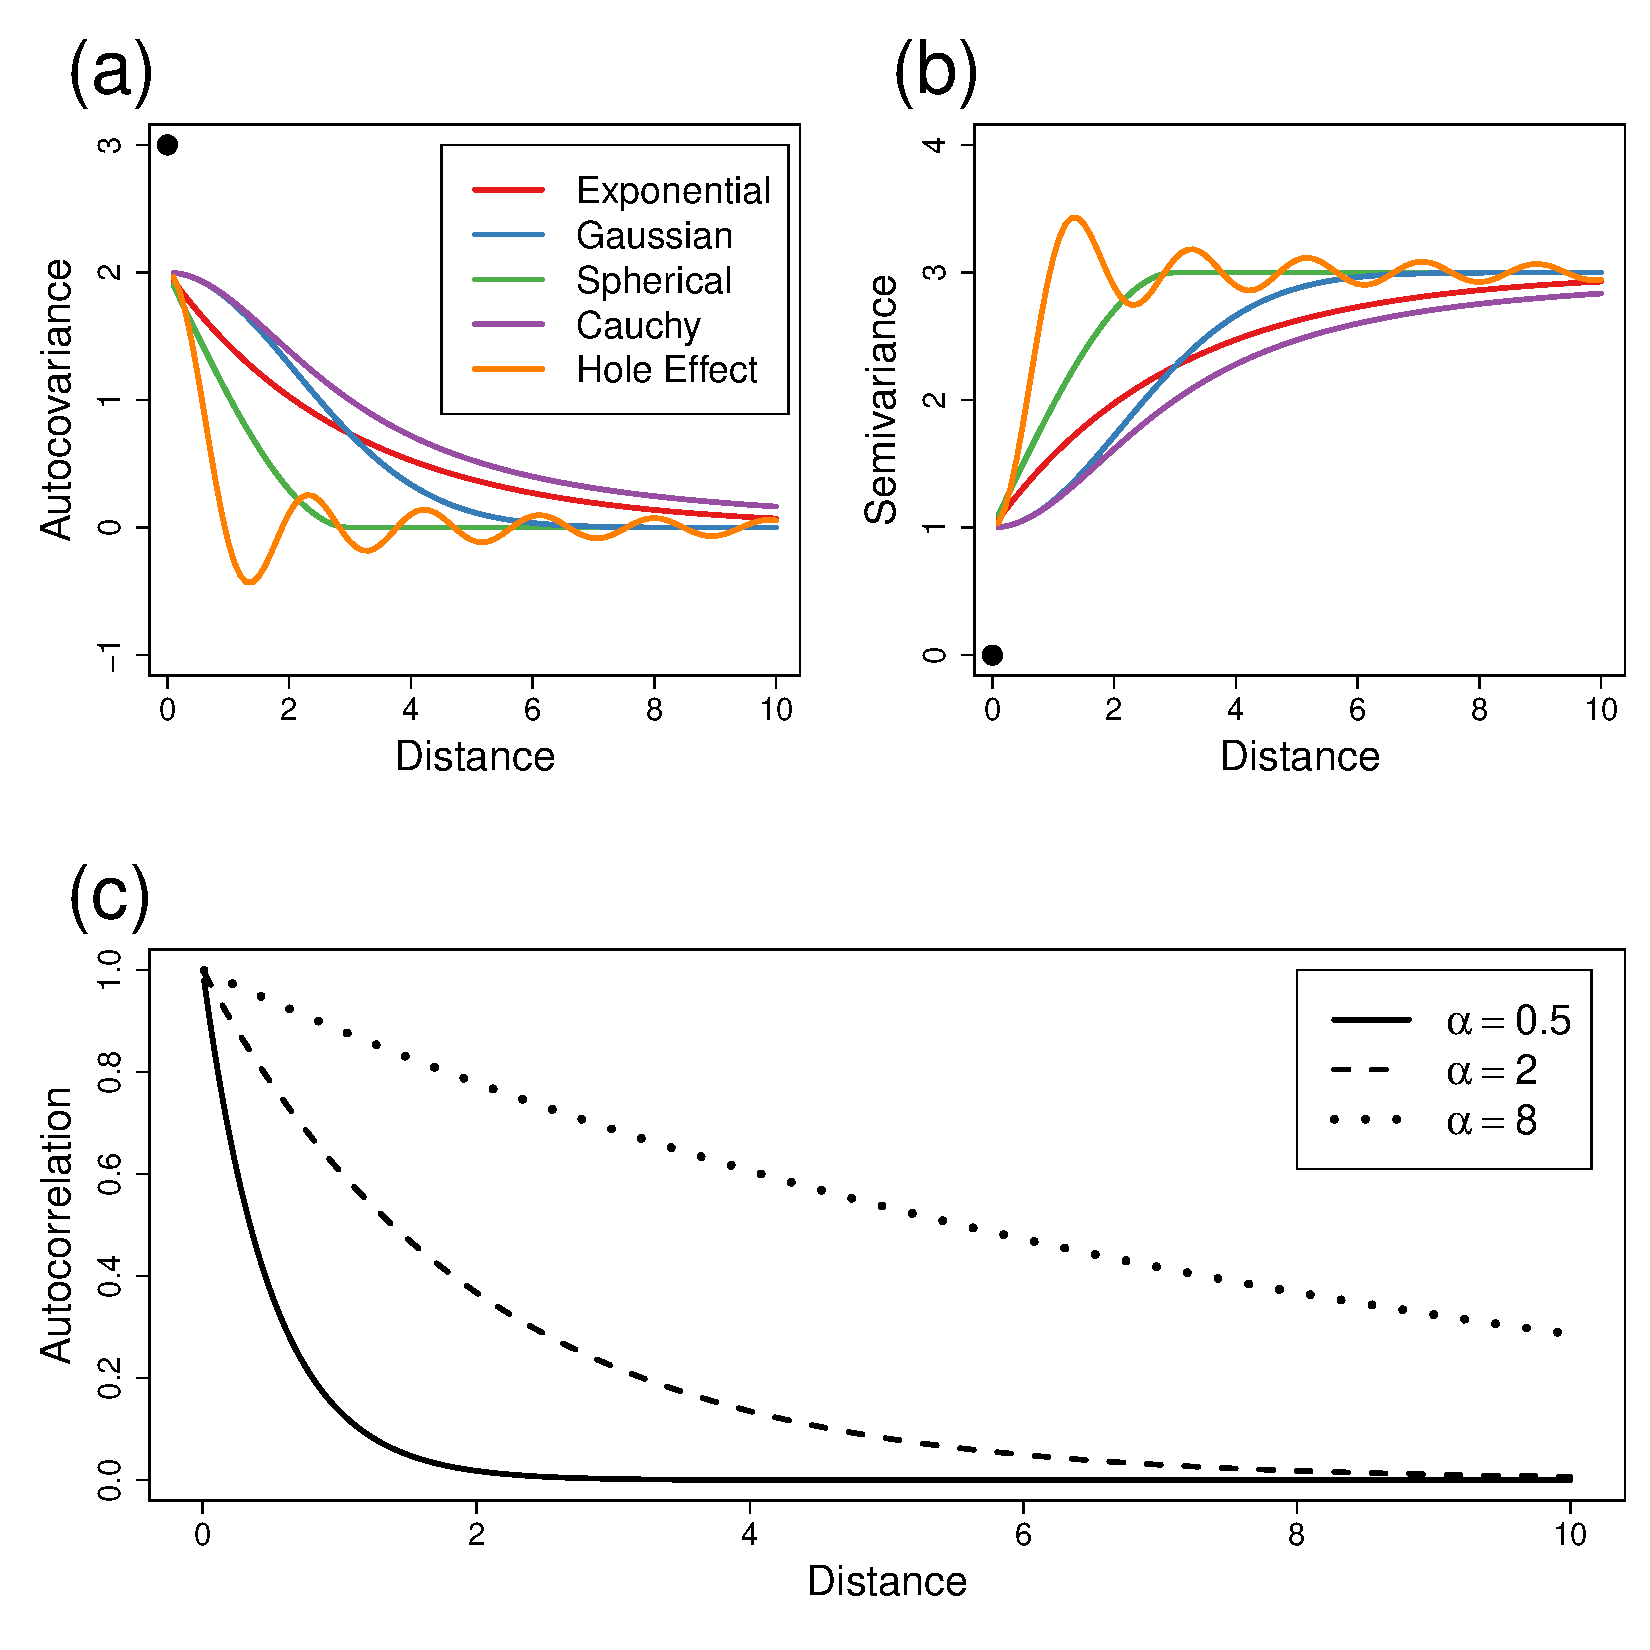
\includegraphics[width=\linewidth]{figure/autocorrModels-1.pdf}
	  \end{center}
	  \caption{Autocorrelation models. (a) Autocovariance functions for various models, with a partial sill of 2 and a nugget effect of 1. (b) The same models as in (a), except represented as semivariogram models. (c) Effect of the range parameter $\alpha$ on autocorrelation functions, where the exponential model was used as an example.  \label{fig:autocorrModels}}
  \end{figure}


%------------------------------------------------------------------------------
%                   CautionEx
%------------------------------------------------------------------------------


	\begin{figure}[H]
	  \begin{center}
	    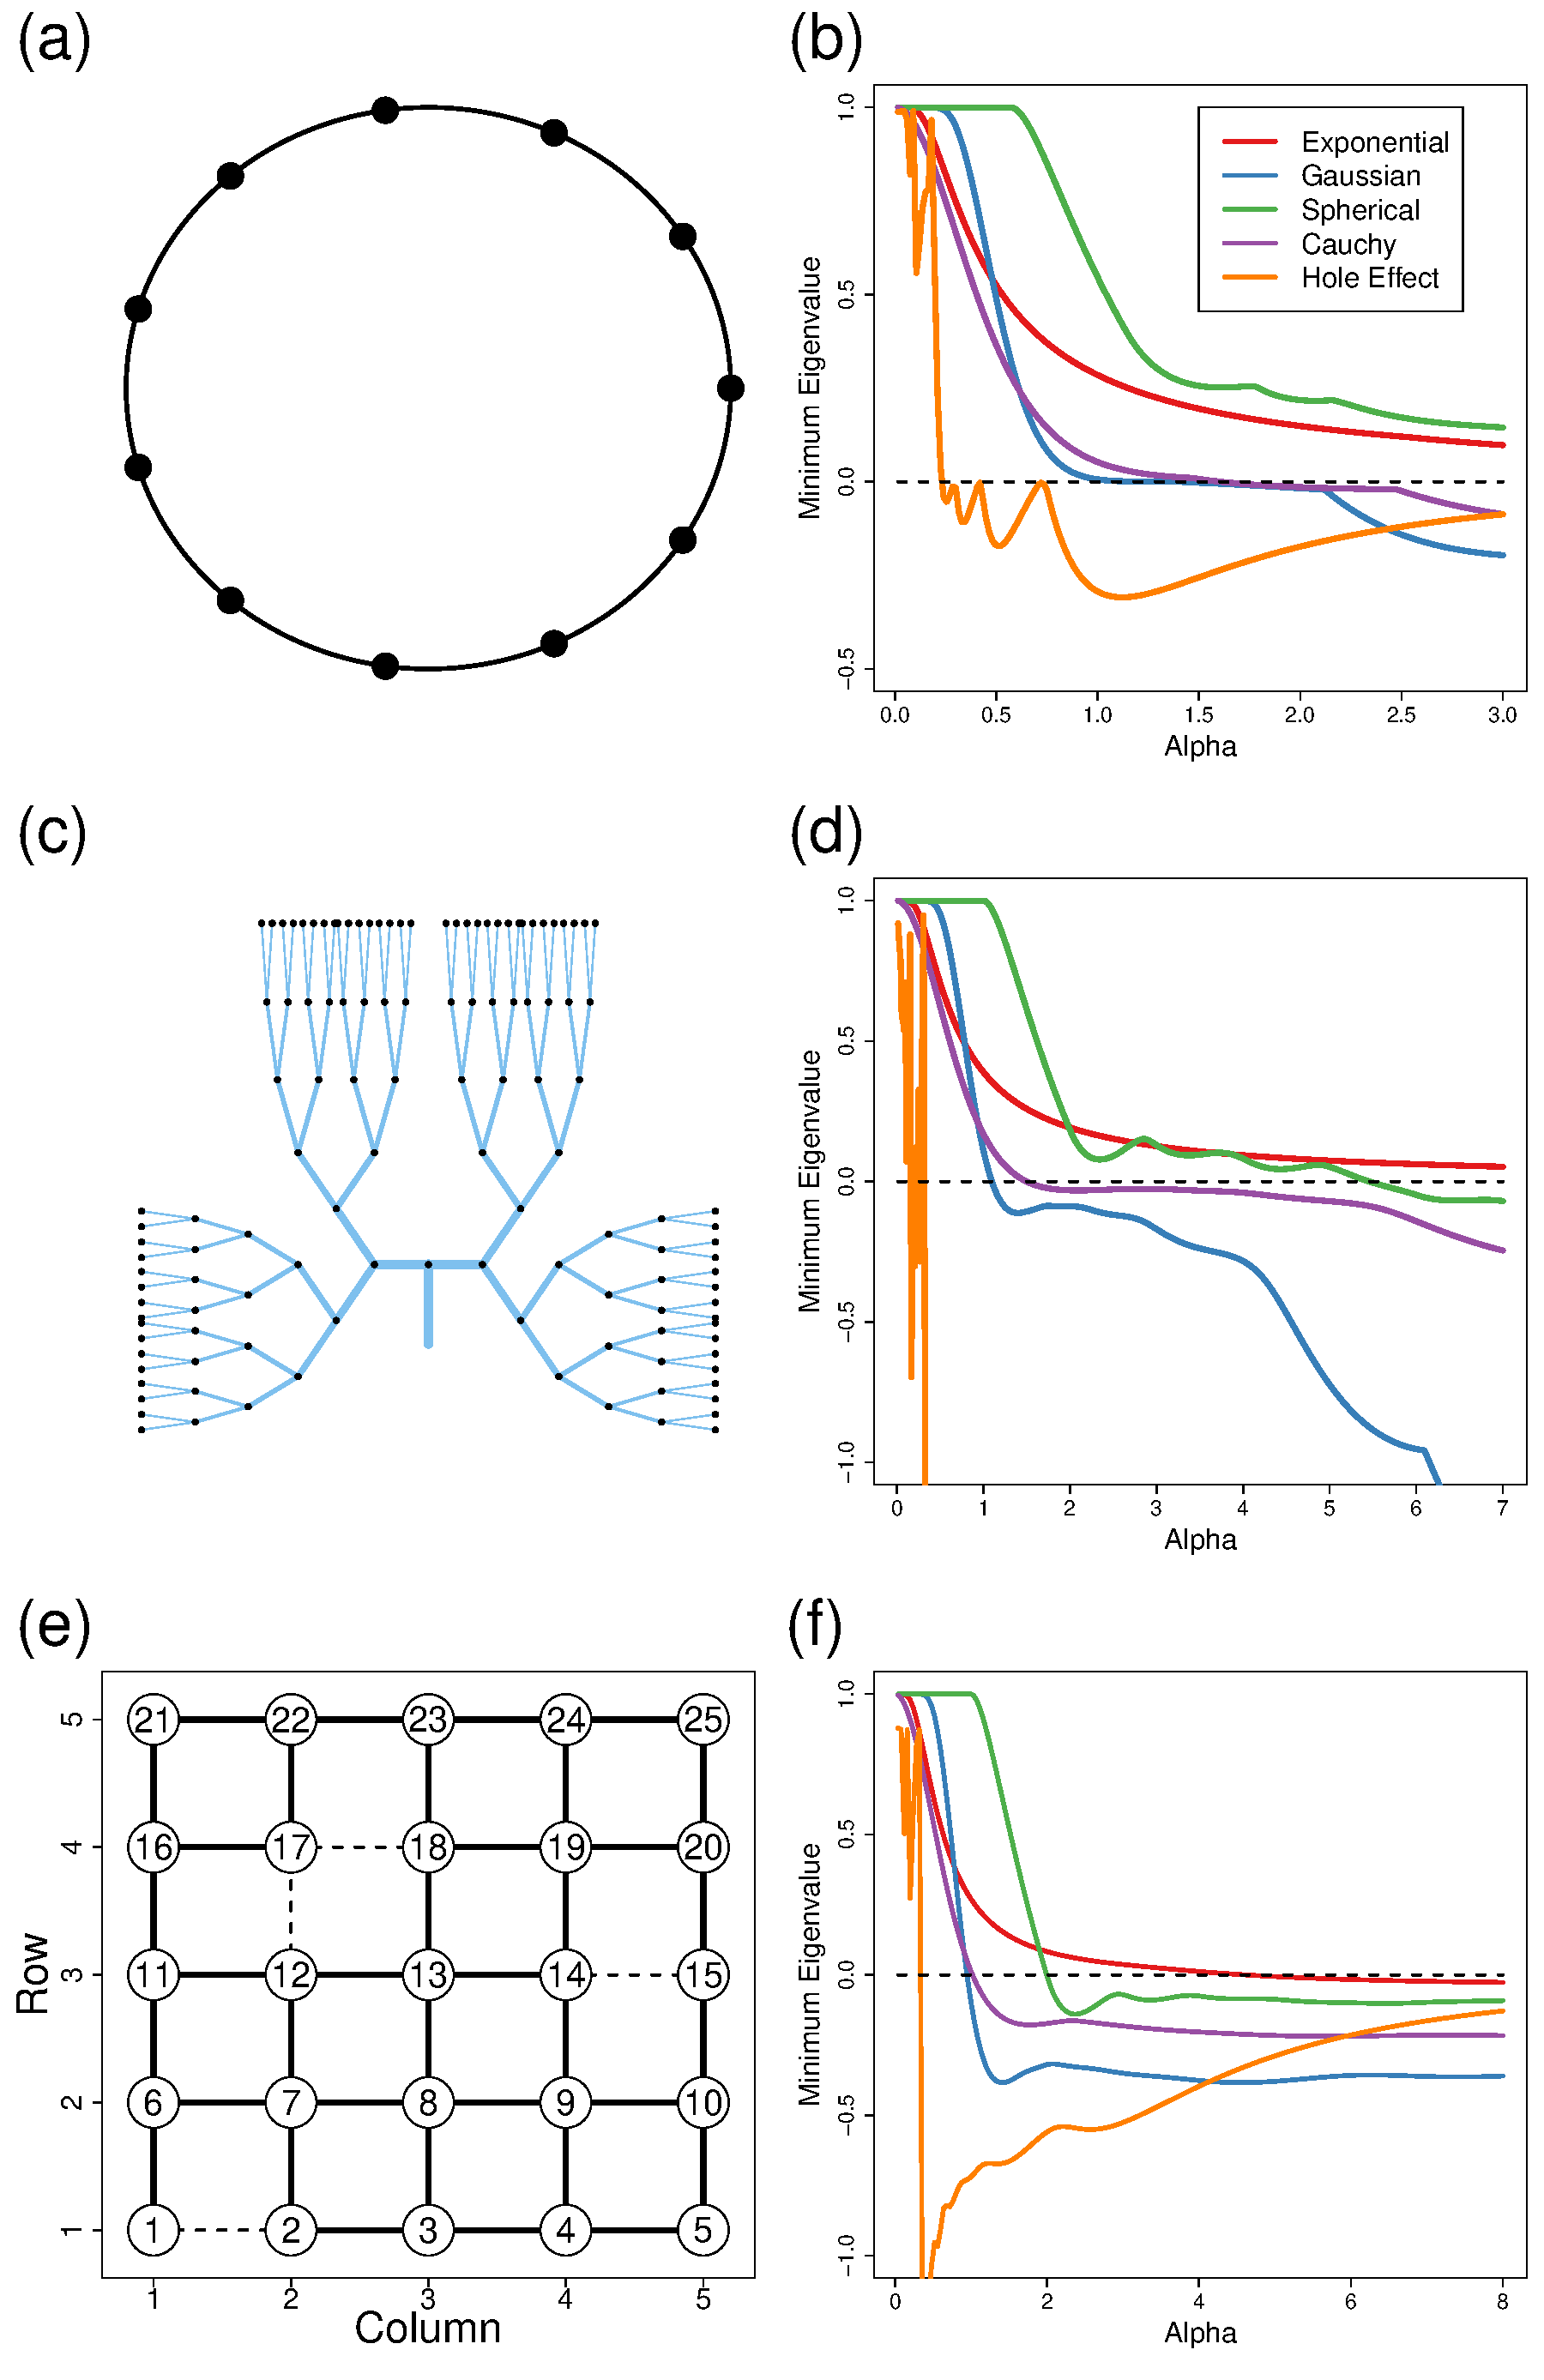
\includegraphics[width=.7\linewidth]{figure/CautionEx-1.pdf}
	  \end{center}
	  \caption{Cautionary examples. (a) 11 spatial locations on a circle are shown with solid circles. (b) Minimum eigenvalue for various autocorrelation models using distances on the circle. (c) A dichotomous branching network (stream) with 127 spatial locations at the node of each branch. (d) Minimum eigenvalue for various autocorrelation models using in-stream distance only. (e) 25 spatial locations on a grid network, where a perfect lattice includes the dashed line, but an irregular lattice includes only the solid lines. (f) Minimum eigenvalue for various autocorrelation models using shortest path distances along the irregular lattice. \label{fig:cautionEx}}
  \end{figure}

%------------------------------------------------------------------------------
%                   realLinDistEigVals
%------------------------------------------------------------------------------


	\begin{figure}[H]
	  \begin{center}
	    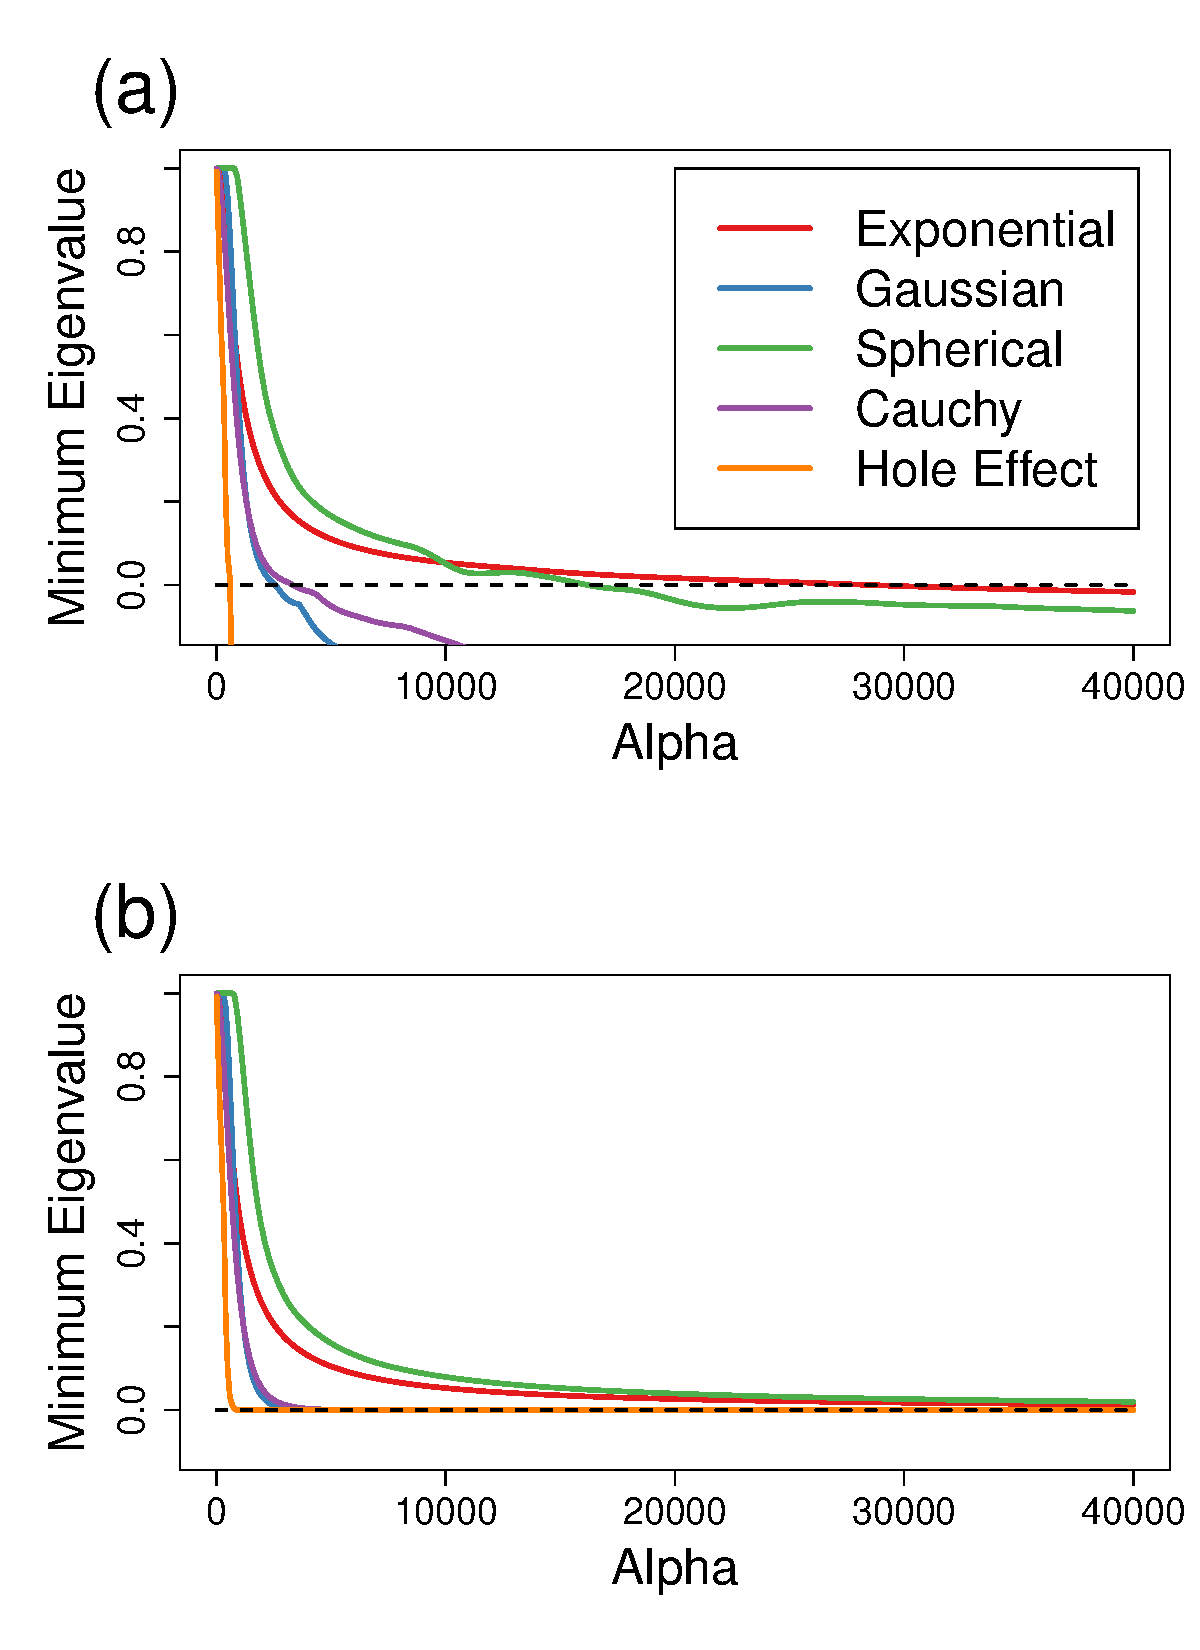
\includegraphics[width=.7\linewidth]{figure/realLinDistEigVals-1.pdf}
	  \end{center}
	  \caption{Minimum eigenvalues for various autocorrelation models for Ladle et al. (2016) data set. (a) Using linear distances among cameras. (b) Using Euclidean distances among cameras.  \label{fig:realLinDistEigVals}}
  \end{figure}

%------------------------------------------------------------------------------
%                   reduRank
%------------------------------------------------------------------------------


	\begin{figure}[H]
	  \begin{center}
	    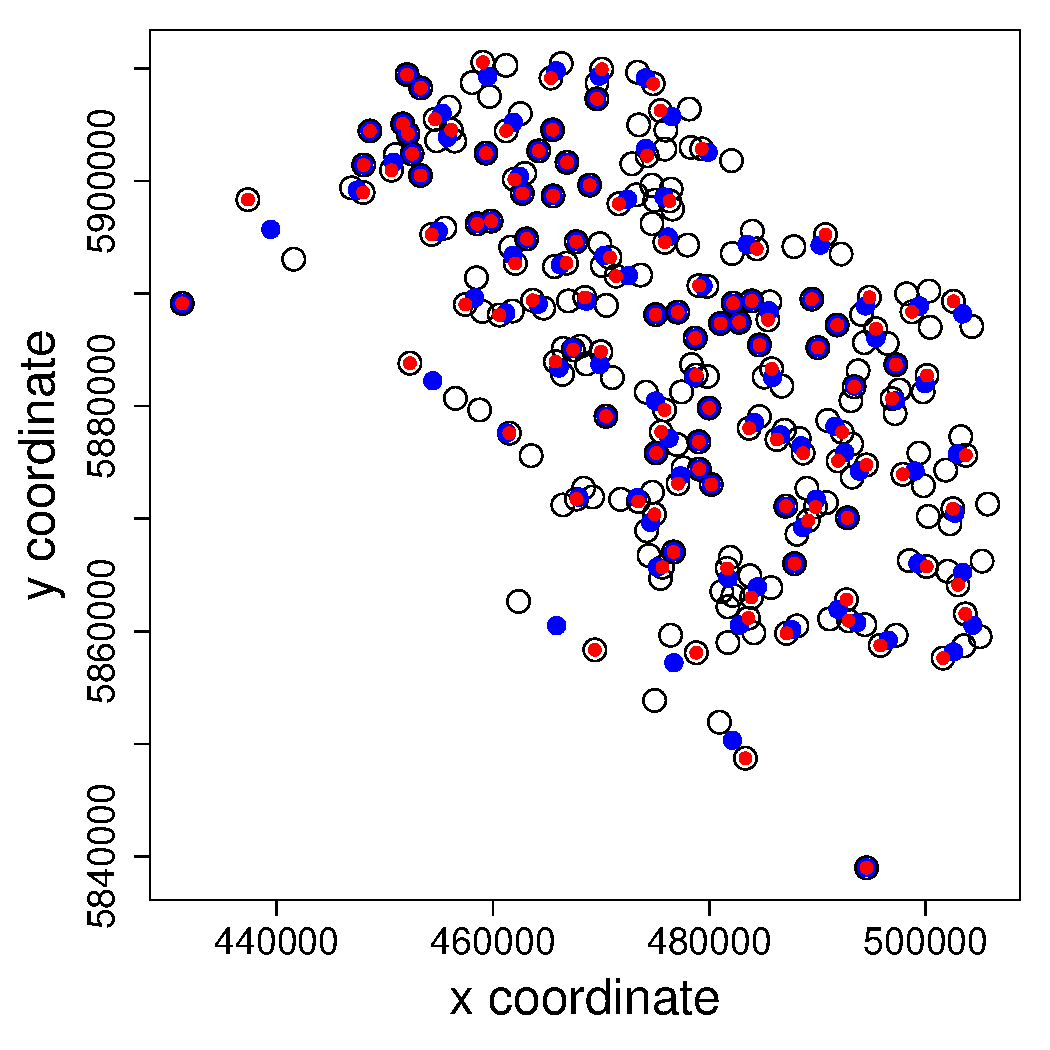
\includegraphics[width=.7\linewidth]{figure/reduRank-1.pdf}
	  \end{center}
	  \caption{All spatial locations (open circles) and knot locations for reduced rank methods.  Initially, k-means on x- and y-coordinates created 120 clusters with center locations given by solid blue circles, and then these were moved to nearest actual locations (solid red circles).   \label{fig:reduRank}}
  \end{figure}

\end{singlespace}


%%%%%%%%%%%%%%%%%%%%%%%%%%%%%%%%%%%%%%%%%%%%%%%%%%%%%%%%%%%%%%%%%%%%%%%%%%%%%%%%%%
%%%%%%%%%%%%%%%%%%%%%%%%%%%%%%%%%%%%%%%%%%%%%%%%%%%%%%%%%%%%%%%%%%%%%%%%%%%%%%%%%%
%%%%%%%%%%%            %%%%%%%    %%%%%%%%  %%%%%%%       %%%%%%%%%%%%%%%%%%%%%%%%
%%%%%%%%%%%  %%%%%%%%%%%%%%%%%  %  %%%%%%%  %%%%%%%  %%%%  %%%%%%%%%%%%%%%%%%%%%%%
%%%%%%%%%%%  %%%%%%%%%%%%%%%%%  %%  %%%%%%  %%%%%%%  %%%%%%  %%%%%%%%%%%%%%%%%%%%%
%%%%%%%%%%%  %%%%%%%%%%%%%%%%%  %%%  %%%%%  %%%%%%%  %%%%%%%   %%%%%%%%%%%%%%%%%%%
%%%%%%%%%%%            %%%%%%%  %%%%  %%%%  %%%%%%%  %%%%%%%%  %%%%%%%%%%%%%%%%%%%
%%%%%%%%%%%  %%%%%%%%%%%%%%%%%  %%%%%  %%%  %%%%%%%  %%%%%%%   %%%%%%%%%%%%%%%%%%%
%%%%%%%%%%%  %%%%%%%%%%%%%%%%%  %%%%%%  %%  %%%%%%%  %%%%%%  %%%%%%%%%%%%%%%%%%%%%
%%%%%%%%%%%  %%%%%%%%%%%%%%%%%  %%%%%%%  %  %%%%%%%  %%%%  %%%%%%%%%%%%%%%%%%%%%%%
%%%%%%%%%%%            %%%%%%%  %%%%%%%%    %%%%%%%       %%%%%%%%%%%%%%%%%%%%%%%%
%%%%%%%%%%%%%%%%%%%%%%%%%%%%%%%%%%%%%%%%%%%%%%%%%%%%%%%%%%%%%%%%%%%%%%%%%%%%%%%%%%
%%%%%%%%%%%%%%%%%%%%%%%%%%%%%%%%%%%%%%%%%%%%%%%%%%%%%%%%%%%%%%%%%%%%%%%%%%%%%%%%%%

\end{flushleft}
\end{spacing}
\end{document}


